\documentclass[12pt]{report}

\usepackage[utf8]{inputenc}
\usepackage[T1]{fontenc}
\usepackage[francais]{babel}
\usepackage{multirow}
\usepackage{array}
\usepackage{color}
\usepackage{stmaryrd}
\usepackage{fancyhdr}
\usepackage{afterpage}
\usepackage{fullpage}
\usepackage{geometry}
\usepackage{setspace}
\usepackage{enumitem}
\usepackage[hyphens]{url}
\usepackage{hyperref}
\usepackage{wrapfig}
\usepackage{float}
\usepackage{graphicx}
\usepackage{tikz}
\usepackage{varwidth}


% Enlève les contours des liens
\hypersetup{
    linkbordercolor={1 1 1},
    citebordercolor={1 1 1},
    urlbordercolor={1 1 1},
    colorlinks=true,
    linkcolor=black,
    urlcolor=blue
}

% Custom colors
\definecolor{green-custom}{HTML}{70ad47}
\definecolor{blue-custom}{HTML}{5b9bd5}

% Redéfinis les marges des tableaux
\let\oldtabular=\tabular
\def\tabular{\small\oldtabular}
\renewcommand{\arraystretch}{1.5}


\title{\textbf{TA72 : Simulation d'atomes}}
\author{
    Aymen DAHECH \\
        \href{mailto:aymen.dahech@utbm.fr}{aymen.dahech@utbm.fr} \and
    Anthony RUHIER \\
        \href{mailto:anthony.ruhier@utbm.fr}{anthony.ruhier@utbm.fr}
}
\date{13 janvier 2017}

\pagestyle{fancy}
\setlength{\headheight}{12pt}
\fancyhf{}
\fancyhead[L]{Aymen DAHECH, Anthony RUHIER}
\fancyhead[R]{Simulation d'atomes}
\geometry{headsep=5ex}

\graphicspath{{graphics/}}
\usetikzlibrary{arrows,positioning}

\setlength{\intextsep}{0pt}

\begin{document}

{
\newgeometry{left=1cm,right=1cm,bottom=3cm,top=1cm}
\begin{titlepage}

\vbox to 70pt{\hfill
\includegraphics[height=2cm]{logo-utbm.eps}}\
\begin{center}

\textsc{\LARGE Université de technologie Belfort-Montbéliard}\\[0.7cm]
\textsc{\LARGE Département Informatique}\\[1.0cm]
\textsc{\Large TA72 -- Projet Tutoré}\\[5cm]


% Title
{ \huge \bfseries Conception d'une simulation d'atomes}\\[0.5cm]
{ \huge \bfseries Rapport général}\\[3cm]

% Author and supervisor
\begin{large}
Aymen \textsc{Dahech} \\
    \href{mailto:aymen.dahech@utbm.fr}{aymen.dahech@utbm.fr}\\[1em]
Anthony \textsc{Ruhier} \\
    \href{mailto:anthony.ruhier@utbm.fr}{anthony.ruhier@utbm.fr}\\[1em]

\end{large}

\vfill

% Bottom of the page
{\large 13 janvier 2017}

\end{center}
\end{titlepage}
}

% Hack to force a new page
{\clearpage\mbox{}\thispagestyle{empty}\clearpage}
\setcounter{page}{1}

\thispagestyle{empty}
\vspace{4em}
\tableofcontents

\afterpage{\cfoot{\thepage}}
\newpage

%%%% Includes des chapitres :
%%%%%%%%%%%%%%%%%%%%%%%%%%%%%%
\setcounter{page}{1}
\chapter*{Introduction}

\addcontentsline{toc}{chapter}{Introduction}

\paragraph{}
Dans le milieu pétrochimique ou dans la chimie pédagogique, nous assistons à
une réelle demande d'outils de simulations d'éléments à vue moléculaire ou
atomique: une représentation graphique d'une réaction permet une meilleure
compréhension de celle-ci, et facilite l'apprentissage en complétant les
maquettes, souvent utilisées.

\paragraph{}
Pour répondre à ce besoin, dans le cadre de notre projet tutoré dans l'Unité de
Valeur TA72, nous avons entamé la conception d'un outil de simulations
graphique d'atomes sous la tutelle de Monsieur Fougères. Nous ne nous
démarrions pas le projet de zéro puisqu'il a également fait l'objet du projet
de fin de semestre de l'UV LP74, suite à laquelle nous nous sommes vus proposer
de le continuer.

\paragraph{}
Tel que laissé en LP74, l'outil affichait une représentation 3D d'un
environnement d'atomes, se déplaçant de manière aléatoire mais gérant les
collisions. L'utilisateur pouvait se déplacer dans l'environnement pour
visualiser les atomes. Quelques problèmes de performances étaient présents,
certains provoquant des crashs de l'application.

\chapter{Présentation du sujet}
\label{presentation_sujet}

\section{Objectifs}

\paragraph{}
Le but du projet a été de continuer le travail entrepris via la première
version de l'application afin d'obtenir trois niveaux de vues (atome, molécule
et réaction), un design en agents et des mouvements d'atomes plus réalistes qui
sont soumis à des lois d'attraction/répulsion


\section{Aperçus}

\paragraph{}
Voici différents aperçus de l'application réalisée :

\begin{figure}[H]
\centering
\centerline{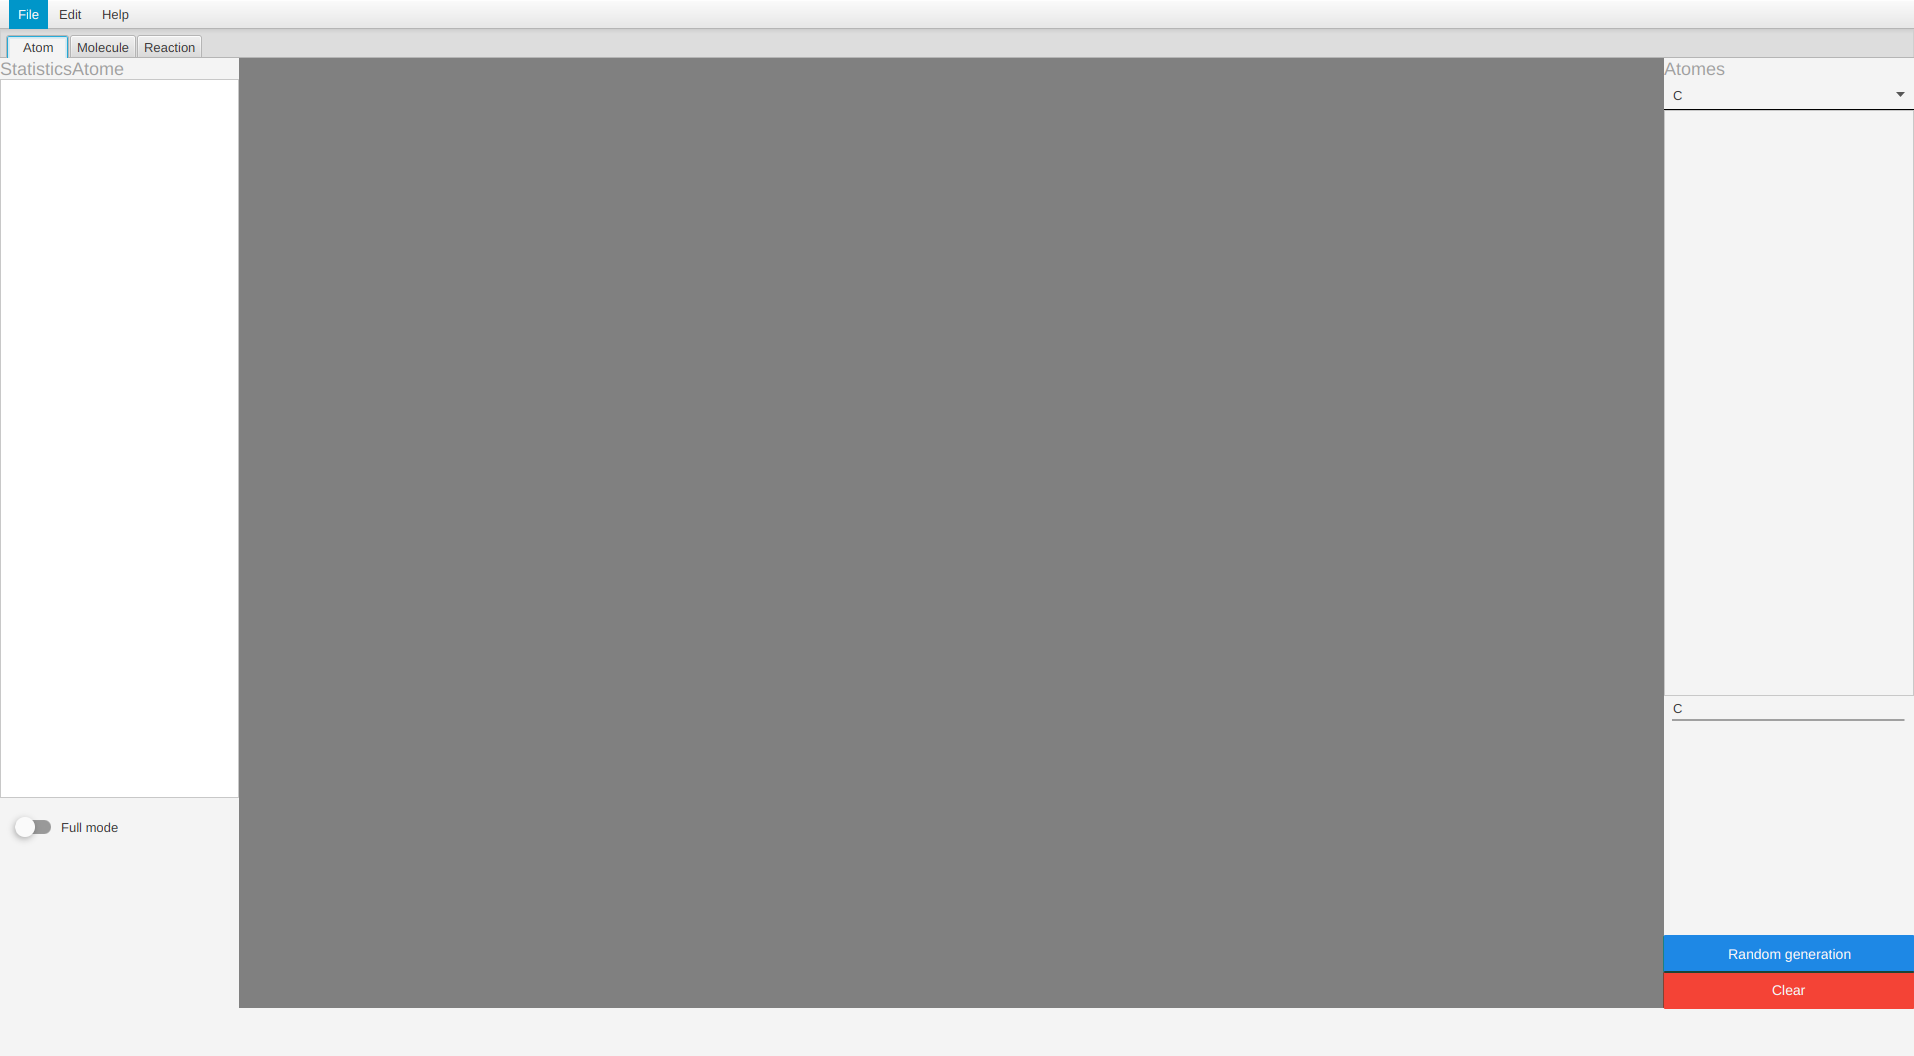
\includegraphics[width=1.2\textwidth]{screenshot_atom}}
\caption{Vue sur l'onglet Atome}
\label{screenshot_atom}
\end{figure}

\paragraph{}
La vue Atome permet normalement de générer un atome et de le visualiser.
Cependant, à la fin de cette TX, il n'est pas encore fonctionnel.

\begin{figure}[H]
\centering
\centerline{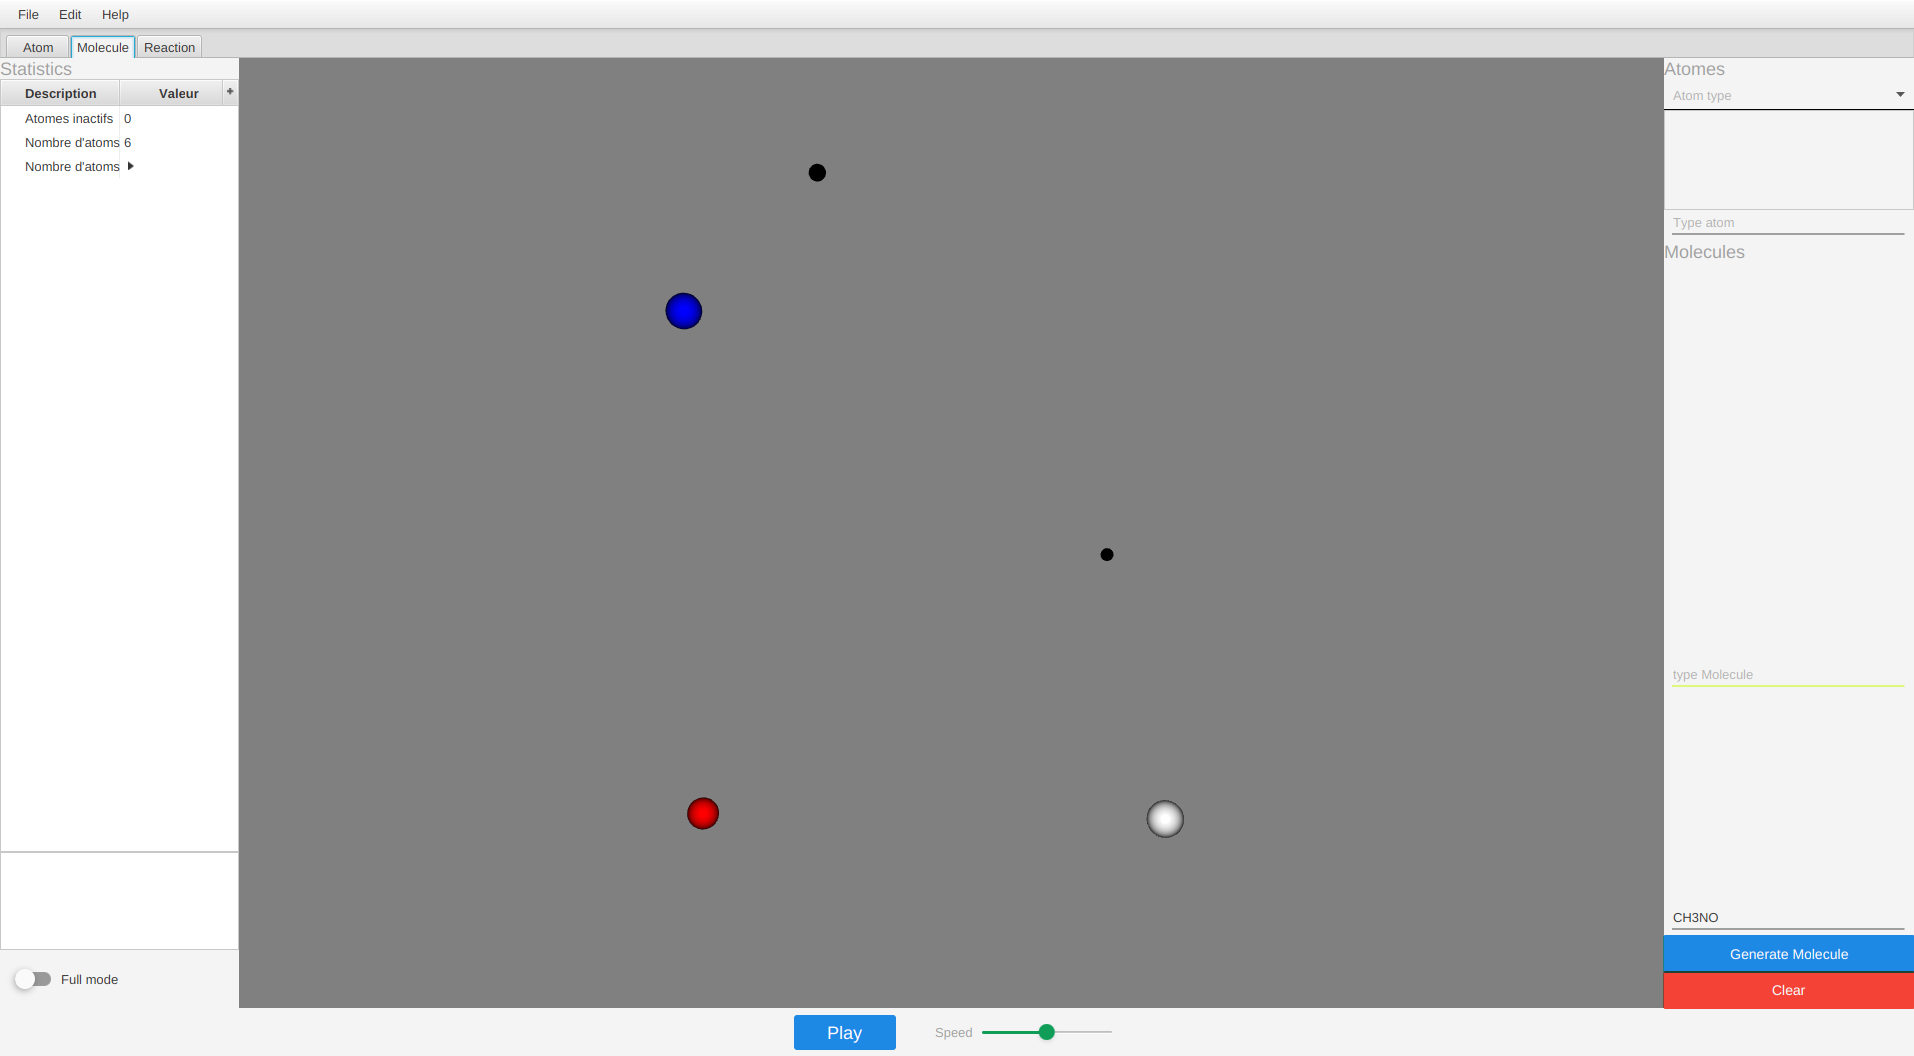
\includegraphics[width=1.2\textwidth]{screenshot_molecule}}
\caption{Vue sur l'onglet Molécule}
\label{screenshot_molecule}
\end{figure}

\paragraph{}
La vue Molécule permet de générer une molécule depuis une formule et de la
visualiser.


\begin{figure}[H]
\centering
\centerline{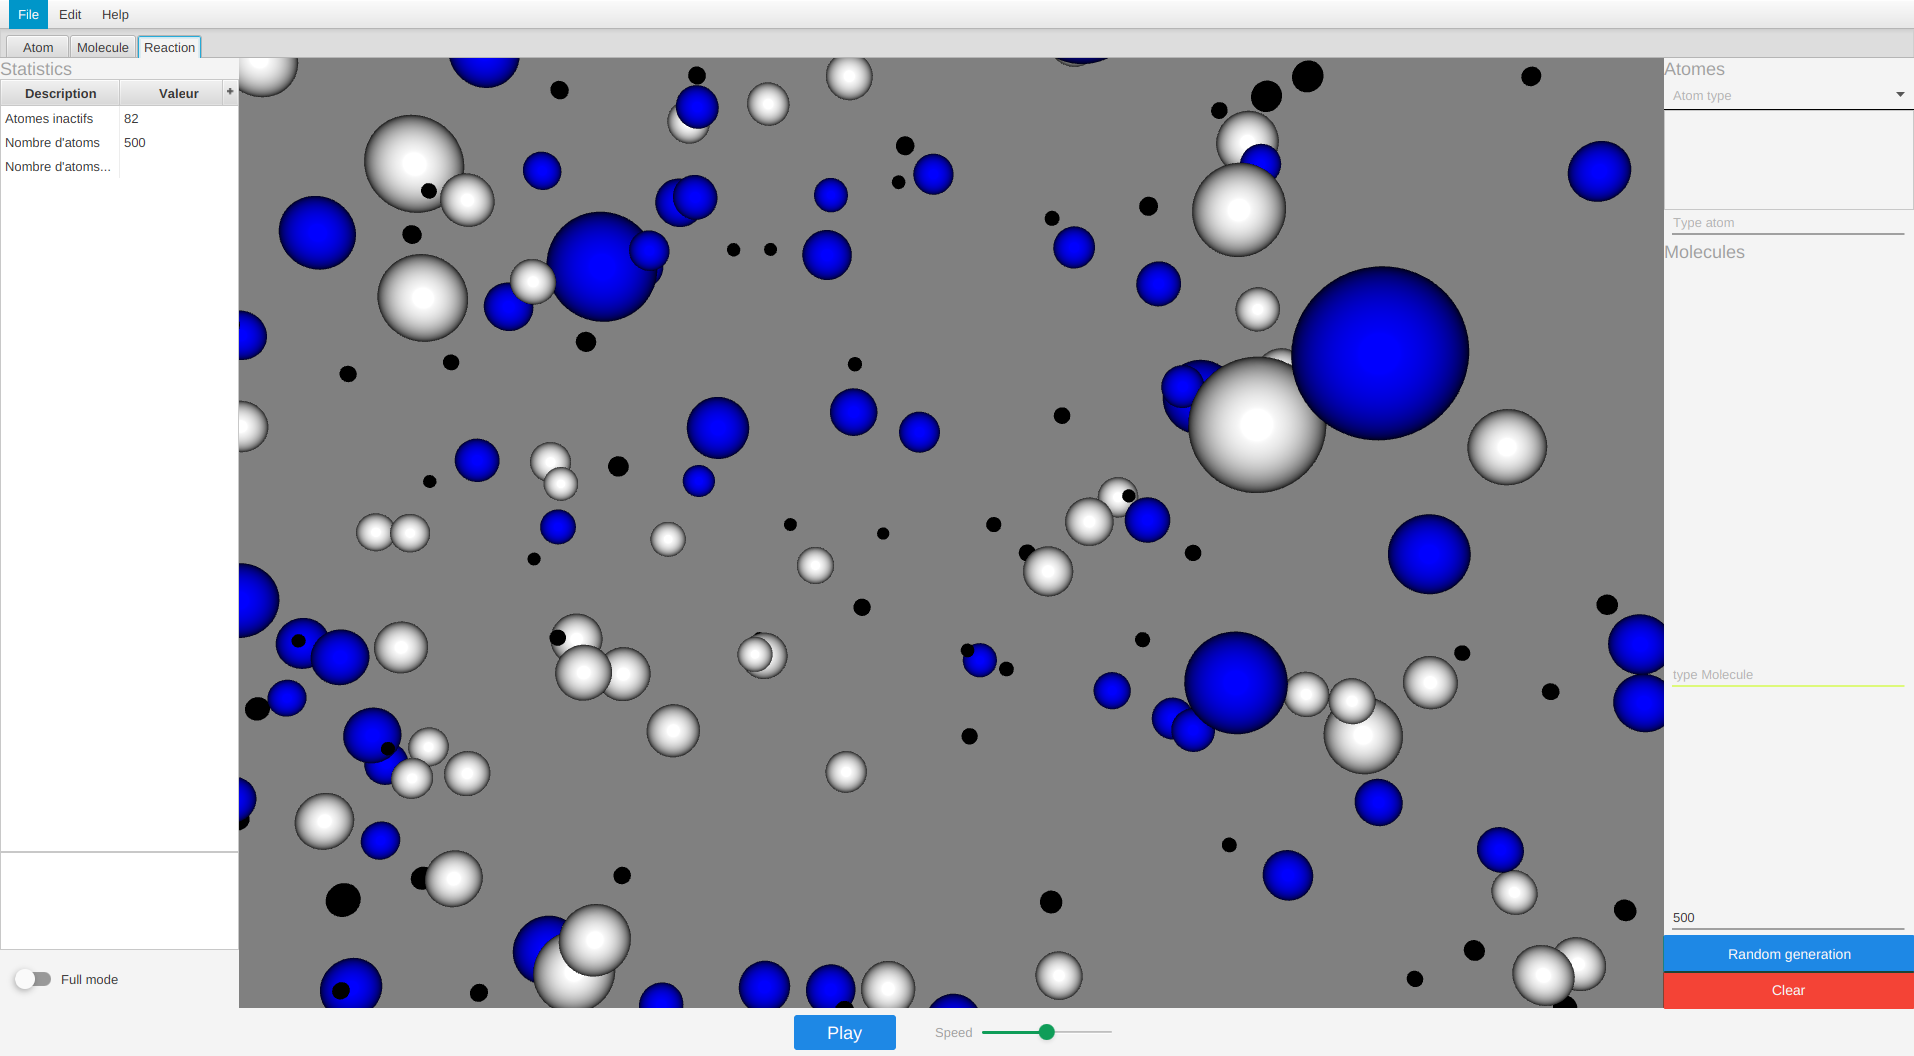
\includegraphics[width=1.2\textwidth]{screenshot_reaction}}
\caption{Vue sur l'onglet Réaction}
\label{screenshot_reaction}
\end{figure}

\paragraph{}
La vue réaction permet de générer un ensemble d'atomes, réagissant ensemble en
formant des molécules via un système d'attraction/répulsion.

\chapter{Mise en oeuvre}
\label{mise_en_oeuvre}

\section{Analyse de l'existant}

\paragraph{}
Dans une optique d'amélioration de l'existant, un bilan sur l'application telle
que rendue en LP74 a été effectué.


\subsection{Application dans un unique thread}

\paragraph{}
Le dessin des atomes, la gestion de leurs déplacements mais ainsi que toute
navigation dans l'interface sont effectués dans un unique thread.

\paragraph{}
Les atomes et molécules sont stockées dans une liste chainée, parcourue de
manière continue et séquentielle par l'application pour mettre à jour leurs
coordonnées. Il est alors nécessaire que le calcul des nouvelles coordonnées
ainsi que le dessin de chaque sphère soient simples et rapides pour rester
inférieur à la durée d'une frame, afin obtenir des mouvements fluides.

\paragraph{}
De cette manière, les atomes n'étaient pas indépendants : un objet
Environnement coordonne l'ensemble, et force de lui-même les mises à jour des
informations.  Il a également comme rôle de vérifier les collisions.


\subsection{Consommation excessive de mémoire}

\paragraph{}
L'application souffre de problèmes de consommation mémoire, avec des fuites
dues à JavaFX (le framework graphique utilisé) qui amènent des lenteurs.
L'application se fige par moments, et il arrive également qu'elle se fasse
tuer par l'OOM killer du système.


\subsection{Mouvement strictement basés sur de l'aléatoire}

\paragraph{}
Les mouvements des atomes ne sont pas basés sur des attractions ou répulsions
entre éléments. L'application impose un aspect ``brouillon'' dans les vecteurs
vitesses des éléments, de façon à donner l'impression que l'environnement n'est
pas uniforme. Tout repose sur un système aléatoire, avec gestion de collisions
et inversions de vecteurs vitesses lorsqu'un élément s'approche de trop près
des bords du bac.


\subsection{Formations de molécules}

\paragraph{}
De façon à former des molécules, et contrairement à ce qui est indiqué dans la
partie liée aux mouvements, une sorte d'attraction a été mise en place. Nous ne
considérons pas que le système en place soit suffisamment exact pour qu'il ait
une réelle influence sur les mouvements des atomes.

\paragraph{}
Néanmoins, si la vitesse d'un atome est suffisamment faible et qu'il rentre en
collision avec un autre atome, ces deux atomes vont se lier. La liaison ne
repose sur rien de scientifique, dans le sens où, par exemple, les couches de
valences ne sont pas prises en compte. Aucune vérification n'est effectuée
pour savoir si les atomes peuvent réellement se lier entre eux.

\chapter{Les modules de la simulation}
\label{les_modules_de_la_simulation}

\definecolor{mygray}{RGB}{208,208,208}
\definecolor{mymagenta}{RGB}{226,0,116}
\newcommand*{\mytextstyle}{\sffamily\Large\bfseries\color{black!85}}
\newcommand{\arcarrow}[3]{%
   % inner radius, middle radius, outer radius, start angle,
   % end angle, tip protusion angle, options, text
   \pgfmathsetmacro{\rin}{1.7}
   \pgfmathsetmacro{\rmid}{2.2}
   \pgfmathsetmacro{\rout}{2.7}
   \pgfmathsetmacro{\astart}{#1}
   \pgfmathsetmacro{\aend}{#2}
   \pgfmathsetmacro{\atip}{5}
   \fill[mygray, very thick] (\astart+\atip:\rin)
                         arc (\astart+\atip:\aend:\rin)
      -- (\aend-\atip:\rmid)
      -- (\aend:\rout)   arc (\aend:\astart+\atip:\rout)
      -- (\astart:\rmid) -- cycle;
   \path[
      decoration = {
         text along path,
         text = {|\mytextstyle|#3},
         text align = {align = center},
         raise = -1.0ex
      },
      decorate
   ](\astart+\atip:\rmid) arc (\astart+\atip:\aend+\atip:\rmid);
}
\begin{tikzpicture}
   \fill[even odd rule,mymagenta] circle (1.5);

   \node at (0,0) [
      font  = \mytextstyle,
      color = white,
      align = center
   ]{
      Atom\\
      Simulator
   };
   \arcarrow{ 85}{3}{ Atomic  }
   \arcarrow{270}{357}{ Molecular }
   \arcarrow{90}{269}{ Reaction }
\end{tikzpicture}
\section{ Module atome : présentation atomique }

\paragraph{}
Le module atome comporte la présentation atomique d'un atome selectionner. La présentation est défini dans un tableau danslequelle est indiqué le type de l'atome, son diametre, le nombre de masse (A) et le nombre atomique (Z).
la présentation d'un atome sous forme d'une sphère. Dans des prochaines amélioration, nous pouvons imaginer avoir autour de l'atome une illustration pédagogique du charge électronique.
\section{ Module molécule : formation des molécules}
\paragraph{}
Dans le module molécule, l'utilisateur peut dans un premier lieu entrer une formule chimique qui sera parser à l'aide des regex.
Une "regular expression" décrit une ou plusieurs chaînes afin de les chercher dans un corps de texte. L'expression sert de modèle pour associer un motif de caractère à la chaîne recherchée.
Une expression régulière consiste en des caractères ordinaires (par exemple, des lettres de a à z) et des caractères spéciaux, appelés métacaractères.


\begin{lstlisting}

 public ArrayList<Atom> parse(Environment environment, String formula, boolean isCHNO) {
        Pattern pattern = Pattern.compile("([A-Z][a-z]?)(\\d*)");//subdivide formula into numbers and letters such as CH2 became C, H2 or NO2Cl N,O2,Cl (the presence of a number means the end of the element)
        Matcher matcher = pattern.matcher(formula);
        ArrayList<Atom> atoms = new ArrayList<>();

        while (matcher.find()) {
            String symbole = matcher.group(2);
            Point3D a_coord;
            if (!verifyCHNO(isCHNO, matcher.group(1))) {
                continue;
}
/.../
\end{lstlisting}
\paragraph{}
Et dans une second temps, l'utilisateur peut utiliser la fonction de drag n drop afin de pouvoir constituer une molécule, les atomes vont etre placer trop proche et dans un environnment réduit, afin que la formation du molécule soit effectuer d'une maniére rapide et efficace.

\section{ Module réaction : Les interactions moléculaires}

\paragraph{}
Les interactions moléculaire sont des forces de répulsion ou d'attraction entre les molécules et les atomes non-liées. L'interaction moléculaire est trés importante dans les domaines des capteurs, conception des médicaments, nanotechnologies, etc. L'interaction moléculaire est connu aussi comme interaction non covalente ou interaction inter-moléculaire. Les interactions moléculaires ne sont pas des liaisons. Les liaisons covalantes  maintients les atomes ensembles dans les molécules . Ces liaisons se rompent et / ou se forment pendant les réactions chimiques


\subsection{Les interactions de Van der waals}
Les interactions moléculaires ont été découvertes par le scientifique néerlandais Vander Waaals. Il a remarqué que les molécules sont collantes.
L'expression «interaction de van der Waals» a signifié des forces cohésives (attraction entre les deux), des forces adhésives (attraction entre différentes) et / ou répulsives entre les molécules.

\begin{table}[h!]
\centering
 \begin{tabular}{||c | c||}
 \hline
 Atom & Van der Waals Radius \\ [0.5ex]
 \hline\hline
 H & 1.2 \\
 \hline
 C & 1.7 \\
 \hline
 N & 1.6 \\
 \hline
 O & 1.5 \\
 \hline
 \end{tabular}
\end{table}
\subsection{La formule de Lennard jones }
La formule de Lennard jones est un modèle mathématique simple qui permet de s'approcher de l'interaction entre les atomes ou des molécules neutres.
L'expression est :
 \begin{displaymath} \phi_{\rm LJ} (r) = 4\varepsilon \left[ \left(\frac{\sigma}{r}\right)^{12} - \left(\frac{\sigma}{r}\right)^{6} \right]\end{displaymath}
Oû
\begin{itemize}
    \item $\varepsilon$ est la profondeur du puit de potentiel
    \item $\sigma$ est la distance finie à laquelle le potentiel entre particule est nulle
    \item r la distance entre les partiqueme
    \item $r_m$ la distance à la quelle le potentiel atteint son minimum
\end{itemize}

A $r_m$, la fonction potentielle a la valeur de $-\varepsilon$
Le potentiel atteint son minimum autour de $r_m = 2^{\frac{1}{6}} \sigma = 1.222 \sigma$ (les distances sont liées)

Ces paramêtres peuvent etre adaptés pour reproduire  des données expérémentales ou des calculs quantique précis.
En raison de sa simplicité de calcul, le potentiel de Lennard jones est largement utilisé dans les simulations informatique meme si des potentiels plus précis existent.
L'application en mode réaction utilise cette formule dans le but de simuler le comportement inter-atomique.

Ce modèle est fortement répulsif à une ditance plus courte que le $1.222 \sigma$.
Le terme  $\sim \frac{1}{r^{12}}$, domine à courte distance, représente le modèle de répulsion entre les atoms lorsqu'ils sont trés proches. Son origine physique est liée au principe de Pauli :  quand les nuages électronique entourant les atomes commencent à ce chevaucher, l'énergie du système augmente brusquement. l'exposant 12 a été choisi exclusivement sur une base protique l'équation est facile à calculer. Sur des bases physiques, un comportement exponentiel serait plus approprié.

Le terme   $\sim \frac{1}{r^{6}}$, domine à large distance, constitue le modèle attractive. C'est le terme qui donne cohésion au système. Une attraction  $\sim \frac{1}{r^{6}}$ est produite par les forces de dispersion de van der waals. Ce sont des interactions plutôt faibles.
Les paramêtres $\sigma$ et $\varepsilon$ sont choisis pour correspondre aux propriétés physiques du matériau.

\underline{Forme simplifié de la formule :}


 \begin{displaymath}
 \phi_{\rm LJ} (r) =  \left[ \left(\frac{A}{r^{12}}\right) - \left(\frac{B}{r^{6}}\right) \right]\end{displaymath}

Oû :
\begin{itemize}
    \item $ A = 4 \varepsilon \sigma ^{12}$
    \item $ B = 4 \varepsilon \sigma ^{6}$
\end{itemize}

\subsection{L'algorithme de Verlet et les lois de Newton}

L'intégration de Verlet est une méthode numérique utilisée pour intégrer les équations de Newotn, il est fréquemment utilisé pour calculer des trajectoires de particules dans des simualtions de dynamique moléculaire et de l'infographie.
Cette intégration fournit une bonne stabilité numérique, ainsi que d'autres propriétés importantes dans les systèmes physiques telque la réversibilité temporelle sans cout de calcul supplémentaire.

\begin{displaymath} {\bf r} (t+\Delta t) = 2{\bf r} (t) - {\bf r} (t-\Delta t) + {\bf a} (t) \Delta t^2 + O(\Delta t^4) \end{displaymath}

Avec

\begin{displaymath} {\bf a} (t) = - (1/m) {\bf\nabla} V\left( {\bf r}(t) \right) \end{displaymath}

Afin de vérifier le bon déroulement de la simulation, l'application doit calculer la somme de l'énergie cinétique K et  V qui doit égale à E  ($ E = K + V $)
\subsection{Le module physique dans l'application}
Chaque atome dans la simulation se déplace simplement en réponse aux forces exercées par les atomes proches et les murs de l'environnement, conformément aux lois du mouvement de Newton. L'algorithme ne connait ni les transformations de phase, ni l'irréversibilité mais ces phénomènes de haut niveau et d'autre émergent de la physique microscopique.

La force entre les atomes est calculée à partir de la formule de Lennard jones.La simulation se rapproche des lois de newton en utilisant l'algorithme de Verlet avec l'étape de temps. L'utilisation d'un pas de temps trop important peut rendre la simulation inexacte et parfois meme instable.
L'application utilise un system naturel d'unité, avec le diamètre atomique, la masse atomique, le profondeur de potentiel de Lennard Jones et la constante de Boltzmann.

\chapter*{Conclusion}

\addcontentsline{toc}{chapter}{Conclusion}

\paragraph{}


\end{document}
